\documentclass[12pt]{article}    
\usepackage{ucs} 
\usepackage[utf8x]{inputenc}
\usepackage[russian]{babel}  
\title{Лабораторная работа №1\\Пружинный маятник}
\author{Хафизов Фанис}
\usepackage[pdftex]{graphicx}

\begin{document}
	\begin{figure}
		\centering
		
\includegraphics[width=0.3\linewidth]{logo}
	\end{figure}
	\maketitle
	\newpage
	\section{Цель работы}
	Целью лабораторной работы является экспериментальное изучение колебаний
	пружинного маятника и ознакомление с методами определения параметров механических колебаний.
	\section{Схема установки}
	\begin{figure}[h]
		\centering
		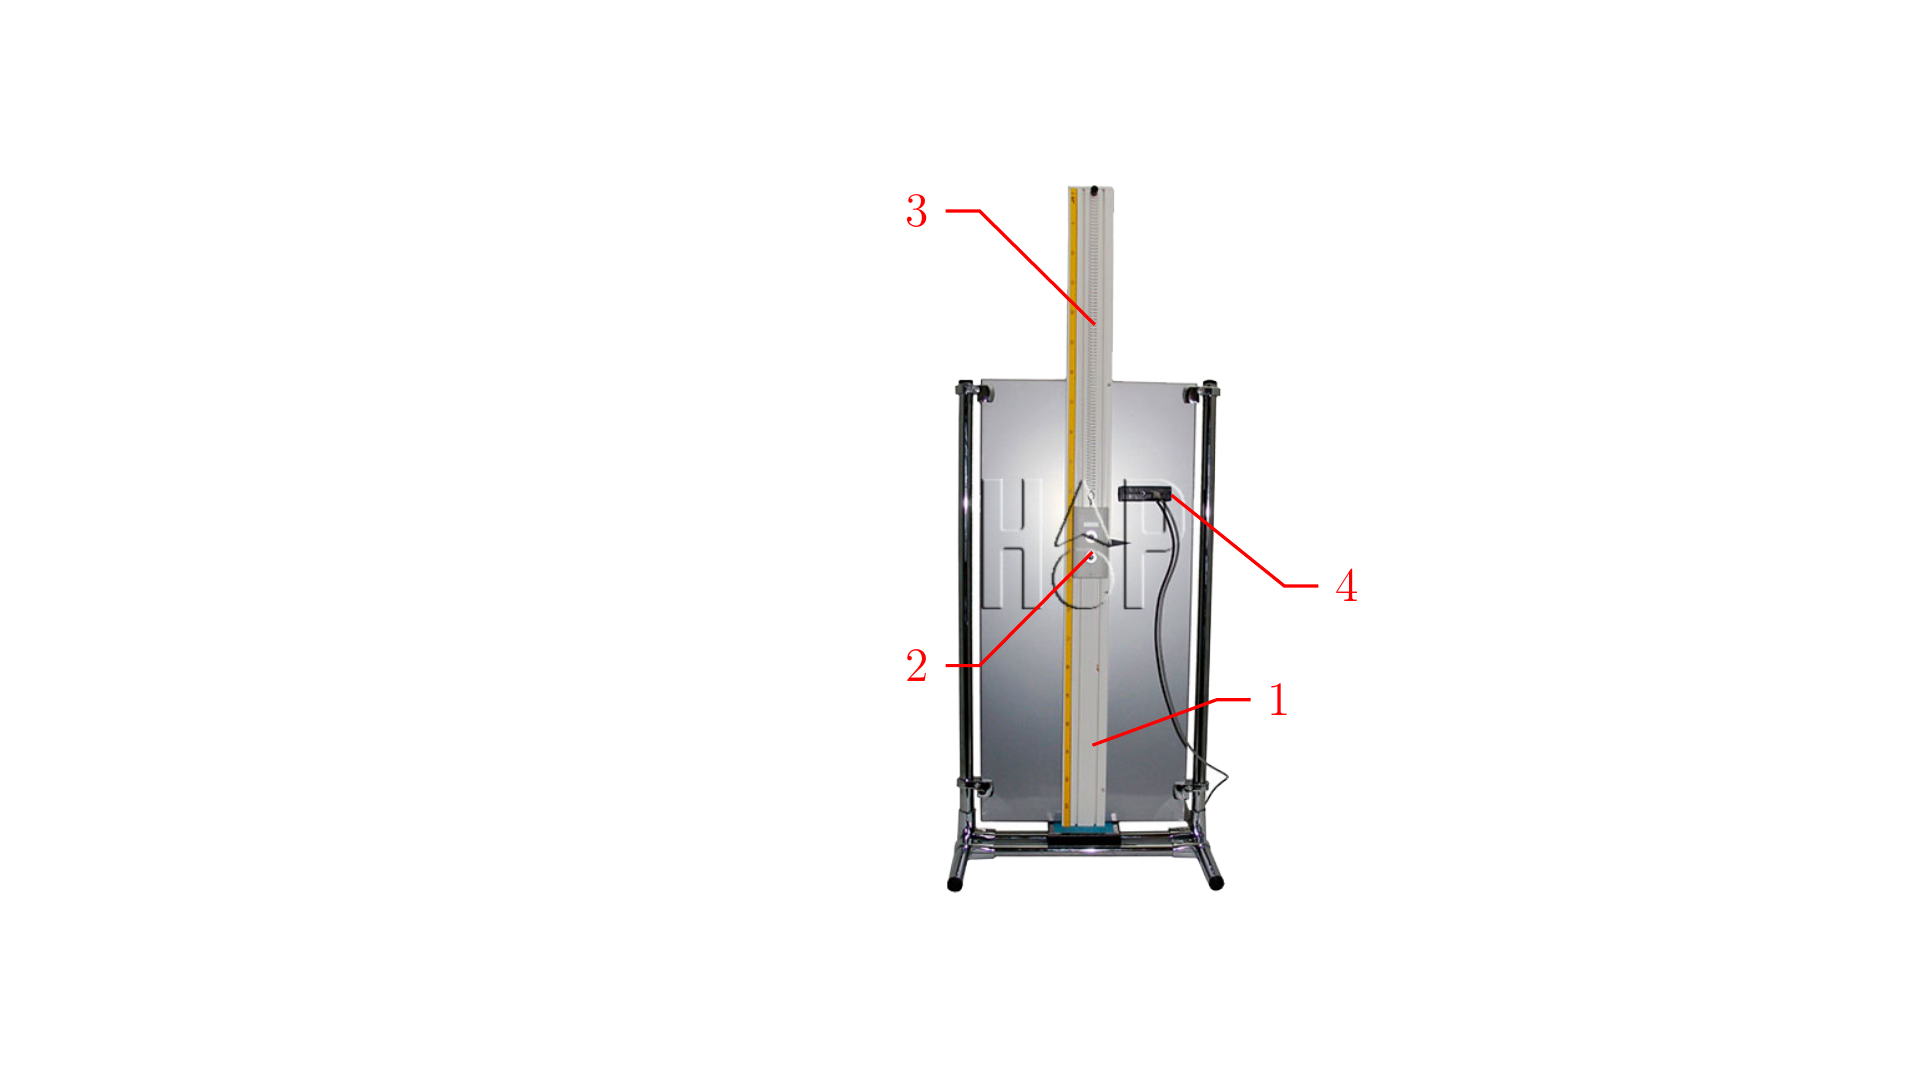
\includegraphics[width=\linewidth]{scheme}
		\caption{Схема установки}
	\end{figure}
Лабораторный стенд (рис. 1) включает в себя вертикальную опорную конструкцию с направляющими пазами (1), а также набор пружин и подвижную каретку
(2), в отверстии которой может фиксироваться дополнительный груз.
К приборам и принадлежностям относятся оптический датчик (4), компьютер с
необходимым программным обеспечением, концентратор для подключения датчика к компьютеру.
\section{Порядок действий}
1)Соберем экспериментальную установку и установим оптический датчик на уровнеx каретки.\\
2)Отведем каретку на небольшое расстояние и отпустим. Запишем результаты нескольких колебаний на компьютере.\\
3)Повторим эксперимент для каретки с грузиком.\\
4)Для нахождения скорости измерим ширину пластины на каретки $l=1{,}4$ см. При каждом перекрытии датчика найдем время прохождения каретки расстояния $l$ и вычислим кинетическую энергию $E_k$. 
\section{Таблица данных и графики}
\begin{figure}[h!]
	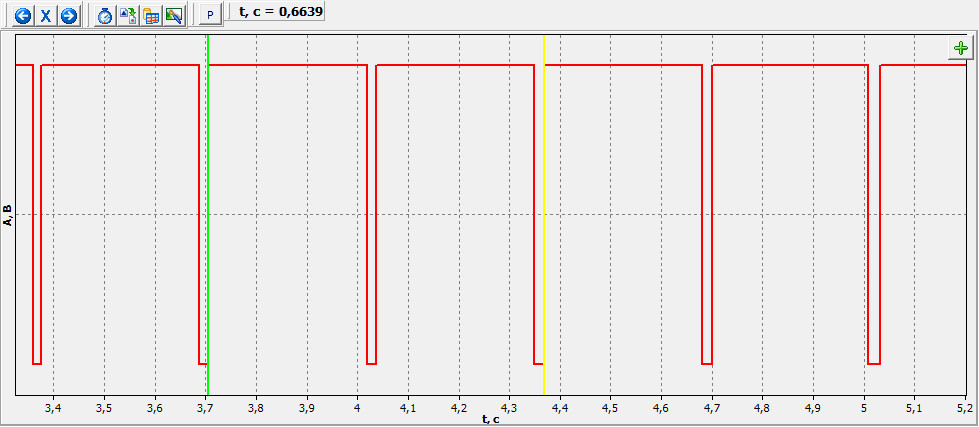
\includegraphics[scale=1.5]{graph1}
	\caption{График для каретки без груза}
\end{figure}
\begin{figure}[h!]
	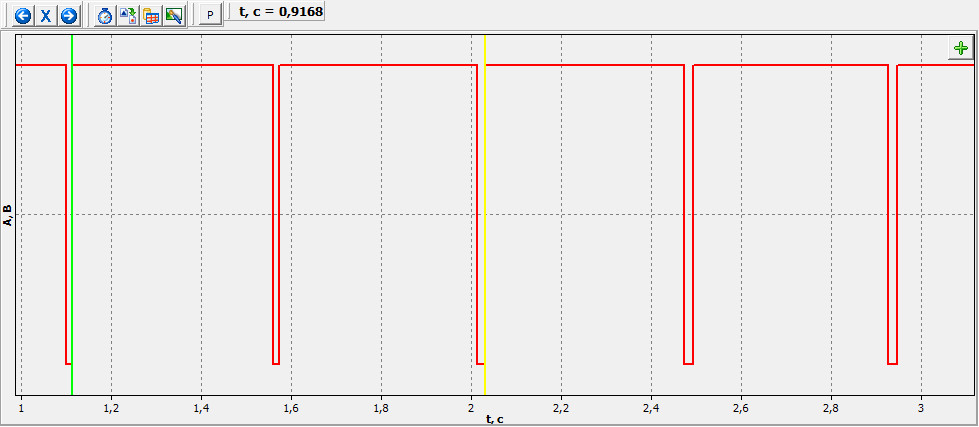
\includegraphics[scale=1.5]{graph2}
	\caption{График для каретки  с грузом}
\end{figure}
\begin{figure}[h!]
	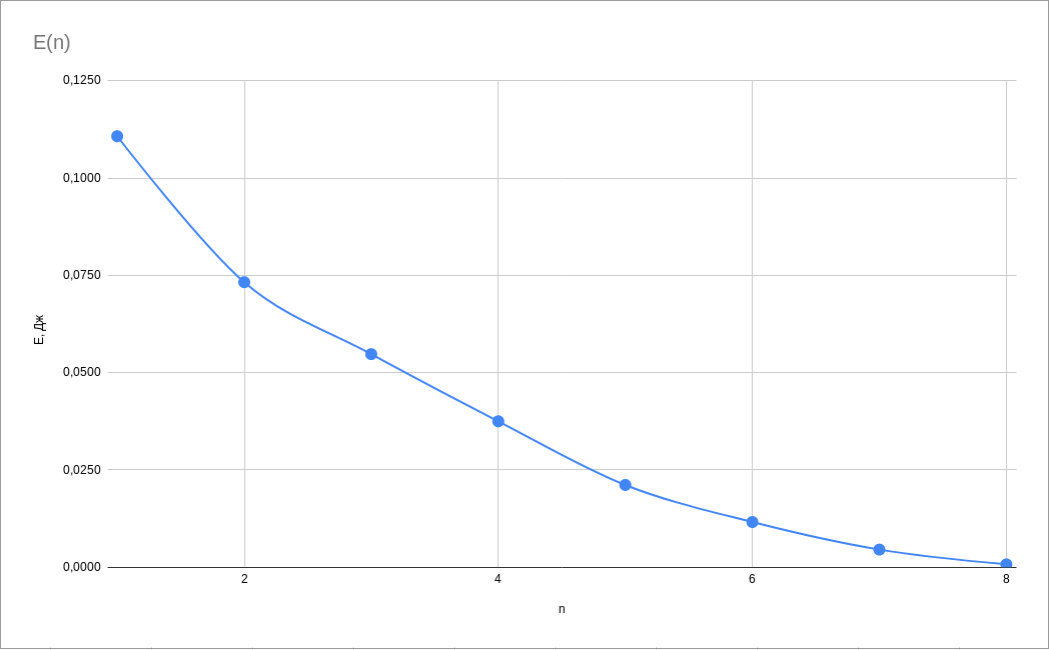
\includegraphics[scale=0.45]{graph3}
	\caption{График зависимости $E_k(n)$}
\end{figure}
\begin{table}[h!]
	\centering
	\begin{tabular}{|c|c|}
		\hline
		$m$, г&$M$, г\\ \hline 
		$102\pm{2}$&$104\pm{2}$\\
		\hline
	\end{tabular}
\caption{Массы грузов}
\end{table}
\begin{table}[h!]
	\begin{tabular}{|l|l|l|l|l|}
		\hline
		$i$, номер & Период маят-   & Средний пе-  & Период маят-          & Средний пе-  \\
		опыта    & ника без груза & риод маятни- & ника с грузом         & риод маятни- \\
		& $T_{i1}$,c           & ка без груза & $T_{i2}$, с                & ка с грузом  \\
		&                & $\overline{T}_1$, с        & \multicolumn{1}{c|}{} & $\overline{T}_2$, с        \\ \hline
		1        & 0,6636         &              & 0,9155                &              \\ \cline{1-2} \cline{4-4}
		2        & 0,6651         &              & 0,9161                &              \\ \cline{1-2} \cline{4-4}
		3        & 0,6639         & 0,6636       & 0,9158                & 0,9163       \\ \cline{1-2} \cline{4-4}
		4        & 0,6623         &              & 0,9172                &              \\ \cline{1-2} \cline{4-4}
		5        & 0,6631         &              & 0,9168                &              \\ \hline
	\end{tabular}
\caption{Пружина 1}
\end{table}
\begin{table}[h!]
	\begin{tabular}{|l|l|l|l|}
		\hline
		n & t, с   & v, м/с & E, Дж  \\ \hline
		1 & 0,0135 & 1,0370 & 0,1108 \\ \hline
		2 & 0,0166 & 0,8434 & 0,0733 \\ \hline
		3 & 0,0192 & 0,7292 & 0,0548 \\ \hline
		4 & 0,0232 & 0,6034 & 0,0375 \\ \hline
		5 & 0,0309 & 0,4531 & 0,0211 \\ \hline
		6 & 0,0417 & 0,3357 & 0,0116 \\ \hline
		7 & 0,0668 & 0,2096 & 0,0045 \\ \hline
		8 & 0,1657 & 0,0845 & 0,0007 \\ \hline
	\end{tabular}
\caption{Значения скорости и кинетической энергии для каждого прохождения мимо датчика}
\end{table}
.\\\\\\\\\\
\section{Расчеты}
$\overline{T}=\frac{\sum\limits_{i=1}^5 T_i}{5}$\\
$\overline{k}=\frac{4\pi^2((m+M)-m)}{\overline{T}_2^2-\overline{T}_1^2}=\frac{4\pi^2M}{\overline{T}_2^2-\overline{T}_1^2}=\frac{4\pi^2\cdot0,104}{0,9163^2-0,6636^2}=10{,}28$ Н/м\\
$\sigma_T=\sqrt{\frac{\sum_{i=1}^5(T_i-\overline{T})^2}{5*4}}$\\
$\sigma_{T1}=0{,}000462$ с\\
$\sigma_{T2}=0{,}000315$ с\\
$\varepsilon_k=\varepsilon_M+\varepsilon_{\Delta \overline{T}^2}=\frac{\Delta M}{M}+\frac{\Delta(\overline{T}_2^2-\overline{T}_1^2)}{(\overline{T}_2^2-\overline{T}_1^2)}=\frac{\Delta M}{M}+\frac{((2\sigma_{T1})^2+\Delta T_1)^2+((2\sigma_{T2})^2+\Delta T_2^2)}{(\overline{T}_2^2-\overline{T}_1^2)}=\frac{0,002}{0,104}+\frac{(2\cdot 0,000462)^2+0,0001^2+(2\cdot 0,000315)^2+0,0001^2}{0,9163^2-0,6636^2}=0{,}02$\\
$\Delta k=\overline{k}\cdot\varepsilon_k=10{,}28\cdot0{,}02=0{,}21$ Н/м\\
$v_i=\frac{l}{t_i}$\\
$E_{ki}=\frac{(m+M)v_i^2}{2}$
\section{Результаты}
$k=(10{,}28\pm0{,}21)$ Н/м, $\delta_k=2\%$\\
\section{Выводы}
Результат получился достаточно точный. Величина относительной погрешности сосставила всего 2\%. Большую часть погрешности составляет приборная погрешность весов при измерении массы груза и каретки. Для увеличения точности эксперимента можно было бы использовать более точные весы и сделать саму установку из более гладких материалов, чтобы уменьшить трение.
\end{document}